\documentclass{beamer}
\title{Assignment 1: Tools}
%\subtitle{}
\author{Joe Lee}
\subject{Tools}
\usetheme{Darmstadt}
\usecolortheme{beaver}
\useoutertheme{infolines}
\useinnertheme{circles}
\usepackage{comment}
\setbeamertemplate{bibliography item}[text]

\setbeamertemplate{footline} { 
  \leavevmode
  \hbox{\begin{beamercolorbox}[wd=.5\paperwidth, ht=2.5ex, dp=1.125ex,
        leftskip=.3cm, rightskip=.3cm plus1fill]{author in head/foot}
      \usebeamerfont{author in head/foot}\insertshortdate
  \end{beamercolorbox}
  \begin{beamercolorbox}[wd=.5\paperwidth,ht=2.5ex, dp=1.125ex, 
        leftskip=.3cm plus1fill, rightskip=.3cm]{title in head/foot}
    \usebeamerfont{title in head/foot}\insertshortauthor
  \end{beamercolorbox}}
  \vskip0pt
}

\begin{document}
\maketitle

%Introduction
\frame{ \transdissolve[duration=0.25] 
  \frametitle{The Team}
  \framesubtitle{Ryan Alcoran, Joe Lee, Shivalik Narad, Nam Phan,
    Swapna Vemparala, Amber Wong}
  \begin{center}
    {\Huge Team Q 06}\\[1em]
  \end{center}
  \pause
  \begin{itemize}
    \item Lee, Joe - Business Manager \pause
    \item Vemparala, Swapna - Project Manager \pause
    \item Wong, Amber - Risk Manager \pause
    \item Narad, Shivalik - Development Manager \pause
    \item Phan, Nam - Development Manager \pause
    \item Alcoran, Ryan - Test Manager
  \end{itemize}
}

%Java
\frame{ \transdissolve[duration=0.25] 
  \frametitle{Language \& Tools}
  {\Huge Java} \pause \\[1em] 
    Object-oriented, \pause similar in syntax to C and C++, \pause 
    but has \pause simpler object model \pause and \pause fewer 
    low-level facilities.\cite{java} \\[2em] \pause
  {\Huge Tools} \\[1em]
    \pause
    \begin{itemize}
      \item Software Configuration Management: {\bf EGit} \pause 
        and regular, command-line {\bf git} client. \pause
      \item Software Hosting Facility: {\bf Github} \pause
      \item Standalone Bug Tracker: {\bf Codebeamer} \pause
      \item Editor and IDE: {\bf Eclipse} and {\bf Emacs} \pause
      \item  Project Management: {\bf OpenProj} \pause
    \end{itemize}
}

%Egit
\frame{ \transdissolve[duration=0.25] 
  \frametitle{Software Configuration Management (SCM)}
  \framesubtitle{Tracking and controlling changes in software}
  {\Huge EGit} \\[1em] \pause 
    ``The EGit project is implementing Eclipse tooling on top of a Java
    implementation of Git.''\\[2em] \pause
    \begin{itemize}
      \item free, open source, designed for branching and merging
      \item decentralized model (everyone has own copy of repository,
        which can later be merged)     
      \item Can be integrated into Eclipse, using a plug-in.
    \end{itemize}
}

%Egit comparison
\frame{ \transdissolve[duration=0.25] 
  \frametitle{Software Configuration Management (SCM)}
  \framesubtitle{Tracking and controlling changes in software}
    {\Huge EGit vs Others} \\[1em] \pause
    {\Large Subversion} \pause
    \begin{itemize}
      \item free, open source, actively developed
      \item easier to use than Git (more tools available for
        non-technical users, error messages are easier to understand)
      \item centralized model (everyone has a working copy and changes
        are submitted to central repository) \pause
    \end{itemize}

    {\Large LibreSource} \pause
    \begin{itemize}
    \item free, open source, maintained and new features under
        development
    \end{itemize}
}

%Egit Installation
\frame{ \transdissolve[duration=0.25] 
  \frametitle{Software Configuration Management (SCM)}
  \framesubtitle{Tracking and controlling changes in software}
    {\Huge EGit Installation} \\[1em] \pause
    \begin{figure}[h!]   
      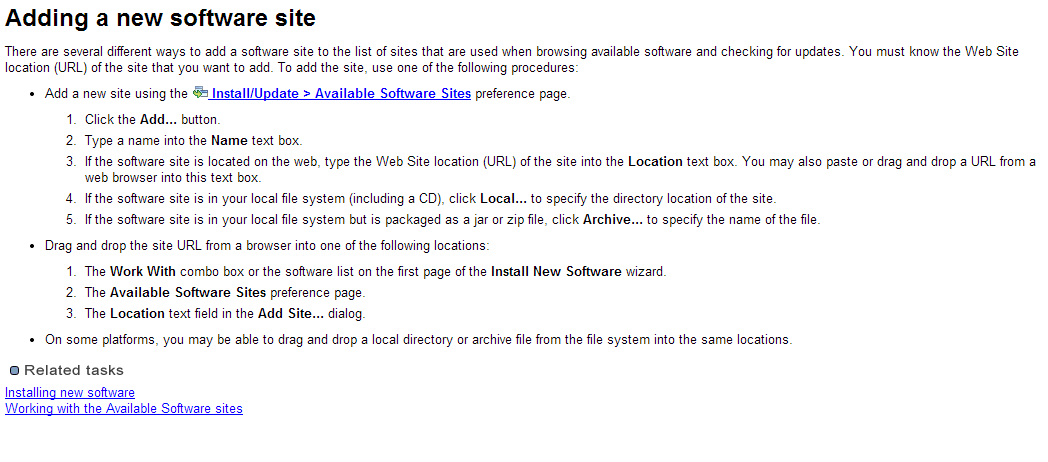
\includegraphics[width=0.8\textwidth]{Screenshots/egit/egit1.png}
      \caption{Instruction to install Egit into Eclispe}
    \end{figure}
}

\frame{ \transdissolve[duration=0.25] 
  \frametitle{Software Configuration Management (SCM)}
  \framesubtitle{Tracking and controlling changes in software}
    {\Huge EGit Installation} \\[1em]
    \begin{figure}[h!]   
      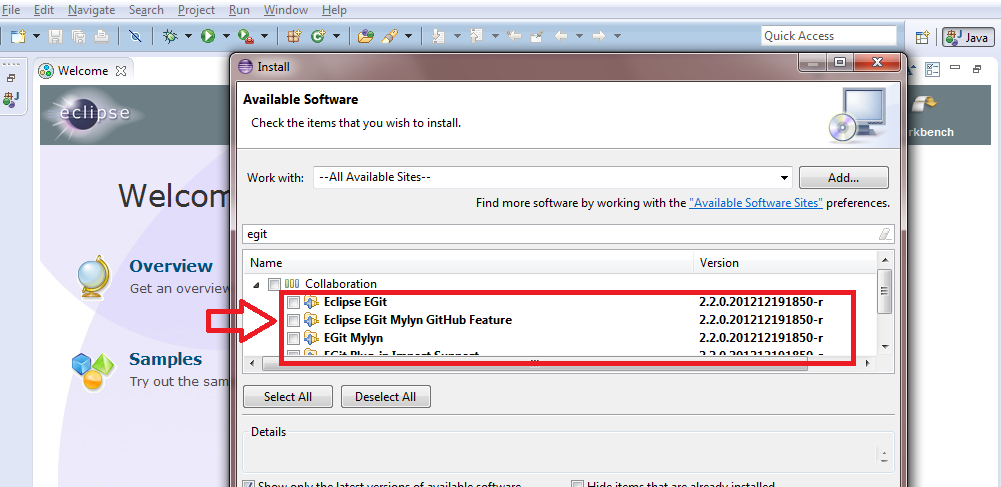
\includegraphics[width=0.8\textwidth]{Screenshots/egit/egit2.png}
      \caption{Instruction to install Egit into Eclispe}
    \end{figure}
}

%Github
\frame{ \transdissolve[duration=0.25] 
  \frametitle{Software hosting facilities}
    {\Huge GitHub} \\[1em] \pause 
    GitHub is a git hosting service. \pause In other words, \pause 
    the company runs git servers for its users. \pause Git is a version 
    control and source code management (SCM) system. \pause \\[1em]

  GitHub is \pause
  \begin{itemize}
    \item Gratis for public projects \pause
    \item Paid for non-public projects.
  \end{itemize}
}

%Github comparison
\frame{ \transdissolve[duration=0.25] 
  \frametitle{Software hosting facilities}
    {\Huge Github vs Others} \\[1em] \pause

    {\Large Google Code} \pause
    \begin{itemize}
      \item Gratis. For ``open source'' projects only. \pause
      \item What is ``open source''? \pause
    \end{itemize}    

    {\Large Tigris} \pause
    \begin{itemize}
      \item Restricted to collaborative software development tools.
    \end{itemize}
}

\frame{ \transdissolve[duration=0.25] 
  \frametitle{Software Configuration Management (SCM)}
  \centering {\Huge Using Git}\\on GitHub's servers
}

\frame{ \transdissolve[duration=0.25] 
    \begin{figure}[h!]   
      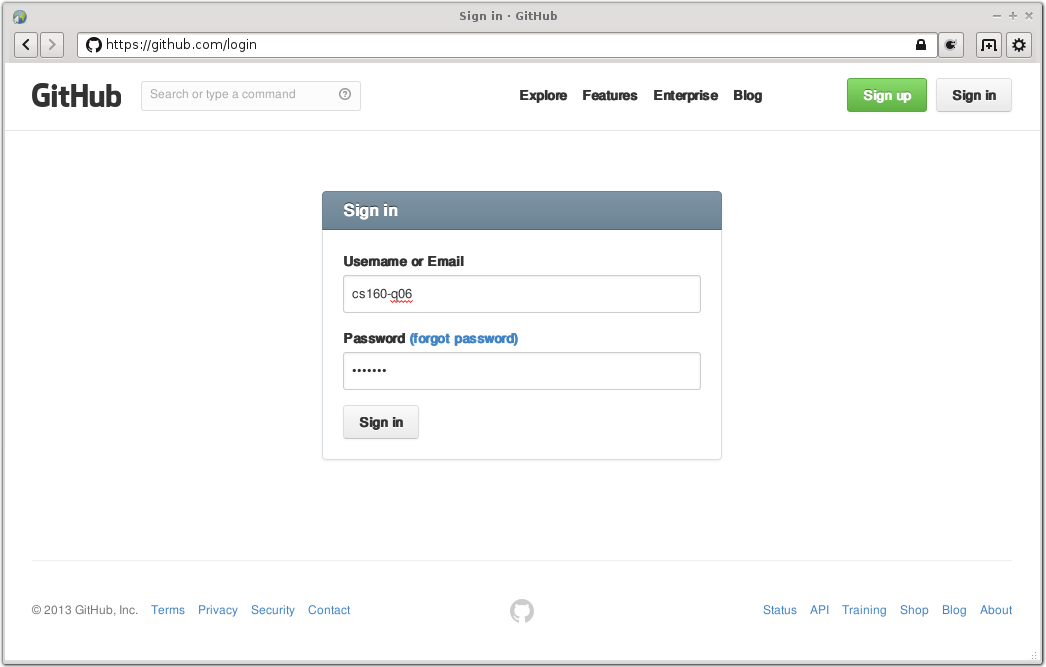
\includegraphics[width=0.8\textwidth]{Screenshots/github/0login.png}
      \caption{GitHub web site login page.}
    \end{figure}
}

\frame{ \transdissolve[duration=0.25] 
    \begin{figure}[h!]   
      \includegraphics[width=0.8\textwidth]{Screenshots/github/1create.png}
      \caption{Create a new git repository.}
    \end{figure}
}

\frame{ \transdissolve[duration=0.25] 
    \begin{figure}[h!]   
      \includegraphics[width=0.8\textwidth]{Screenshots/github/2clone.png}
      \caption{Clone the repository on your own computer.}
    \end{figure}
}

\frame{ \transdissolve[duration=0.25] 
    \begin{figure}[h!]   
      \includegraphics[width=0.8\textwidth]{Screenshots/github/3edit.png}
      \caption{Make edits and add files.}
    \end{figure}
}

\frame{ \transdissolve[duration=0.25] 
    \begin{figure}[h!]   
      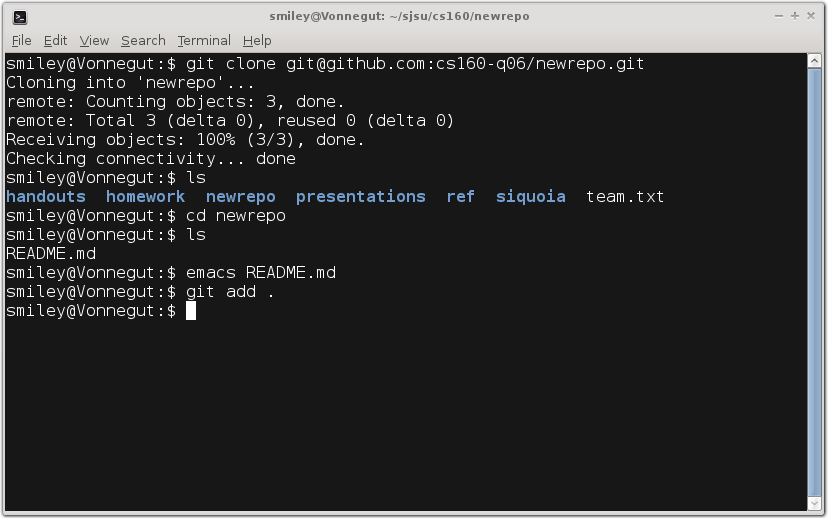
\includegraphics[width=0.8\textwidth]{Screenshots/github/4add.png}
      \caption{Add changed files to your next commit.}
    \end{figure}
}

\frame{ \transdissolve[duration=0.25] 
    \begin{figure}[h!]   
      \includegraphics[width=0.8\textwidth]{Screenshots/github/5commit.png}
      \caption{Commit your changes.}
    \end{figure}
}

\frame{ \transdissolve[duration=0.25] 
    \begin{figure}[h!]   
      \includegraphics[width=0.8\textwidth]{Screenshots/github/6comment.png}
      \caption{Add a commit message to summarize changes.}
    \end{figure}
}

\frame{ \transdissolve[duration=0.25] 
    \begin{figure}[h!]   
      \includegraphics[width=0.8\textwidth]{Screenshots/github/7push.png}
      \caption{Push changes to the repository.}
    \end{figure}
}

%Git client installation
\frame{ \transdissolve[duration=0.25] 
  \frametitle{Software hosting facilities}
    {\Huge GitHub} \\[1em]
    \pause
    \begin{figure}[h!]   
      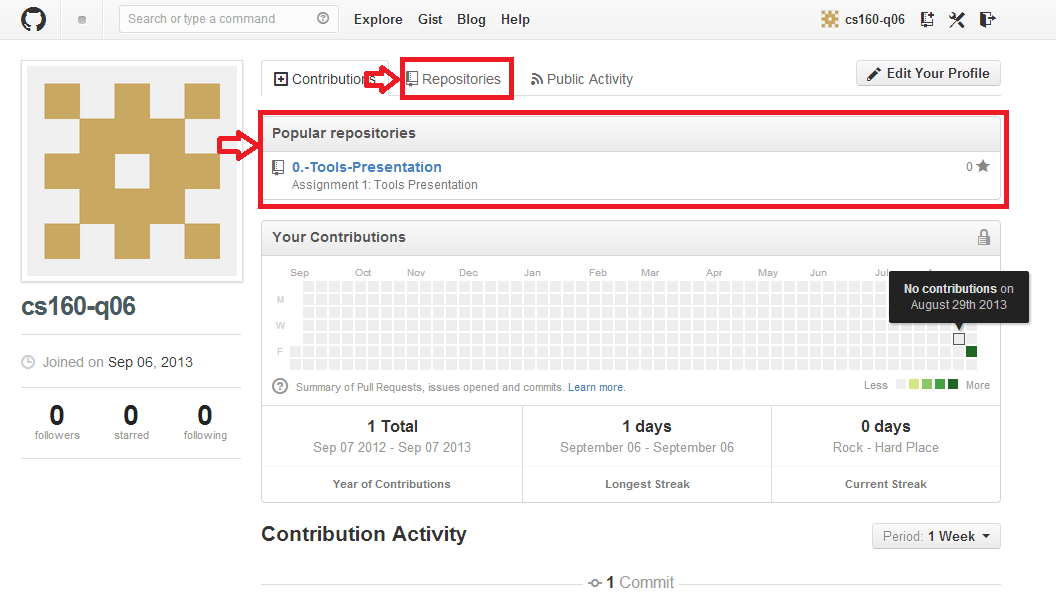
\includegraphics[width=0.8\textwidth]{Screenshots/github/github1.png}
      \caption{GitHub web UI and sample Repository}
    \end{figure}
}

\frame{ \transdissolve[duration=0.25] 
  \frametitle{Software hosting facilities}
    {\Huge GitHub client installation} \\[1em]
   \begin{figure}[h!]   
      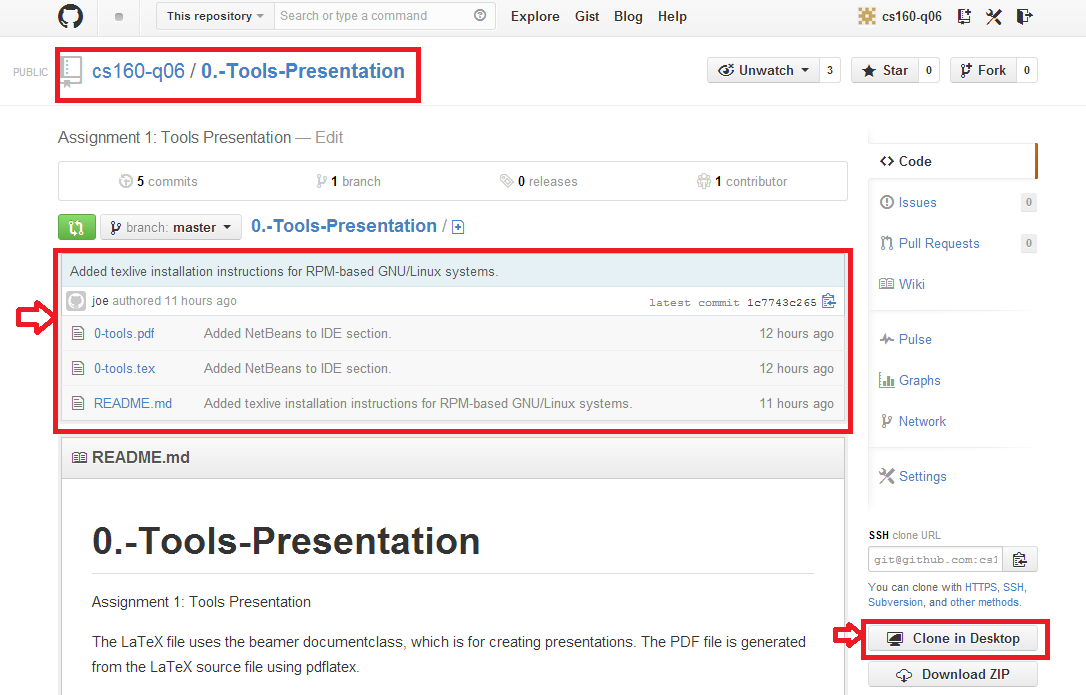
\includegraphics[width=0.7\textwidth]{Screenshots/github/github2.png}
  \caption{Inside a repository and how to clone it}
\end{figure}
}

\frame{ \transdissolve[duration=0.25] 
  \frametitle{Software hosting facilities}
    {\Huge GitHub client installation} \\[1em]
   \begin{figure}[h!]   
      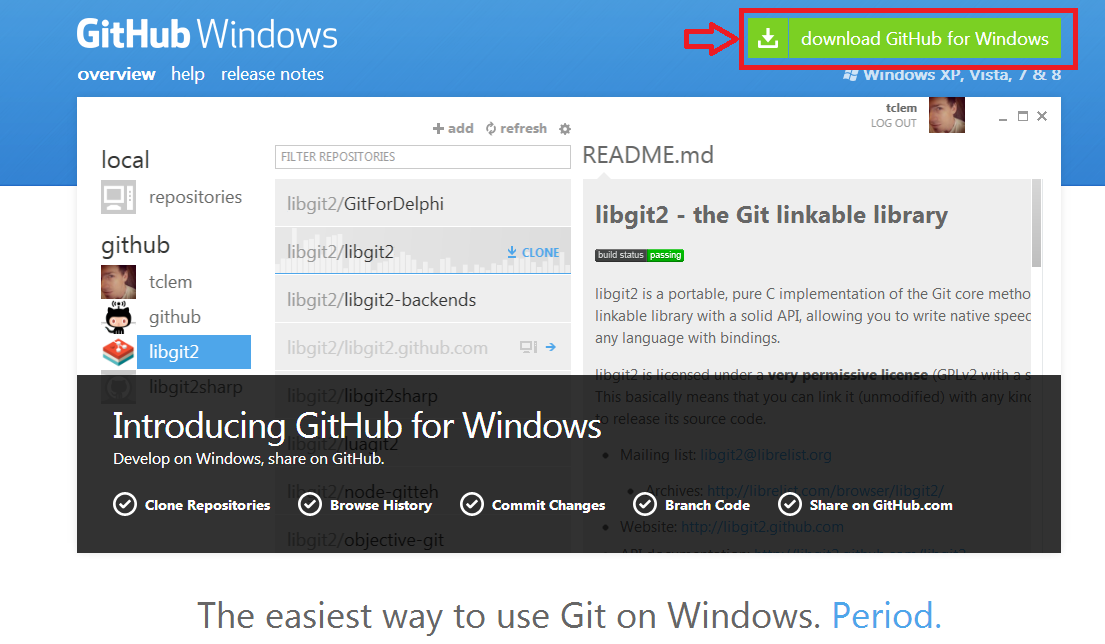
\includegraphics[width=0.7\textwidth]{Screenshots/github/github3.png}
  \caption{Github software for Windows}
\end{figure}
}

\frame{ \transdissolve[duration=0.25] 
  \frametitle{Software hosting facilities}
    {\Huge GitHub client installation} \\[1em]
   \begin{figure}[h!]   
      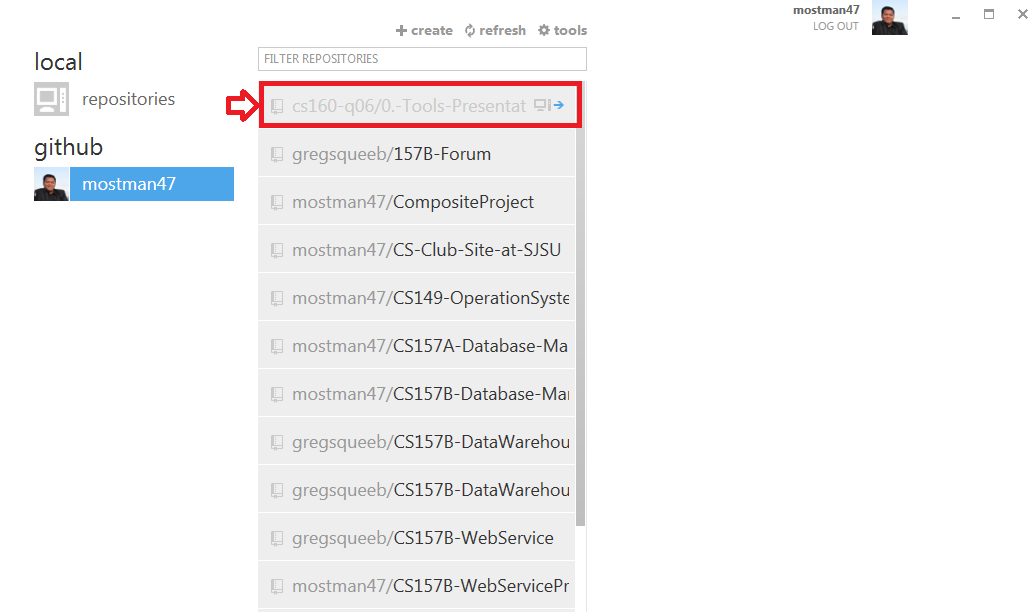
\includegraphics[width=0.7\textwidth]{Screenshots/github/github7.png}
  \caption{Github software UI}
\end{figure}
}

\frame{ \transdissolve[duration=0.25] 
  \frametitle{Software hosting facilities}
    {\Huge GitHub client installation} \\[1em]
   \begin{figure}[h!]   
      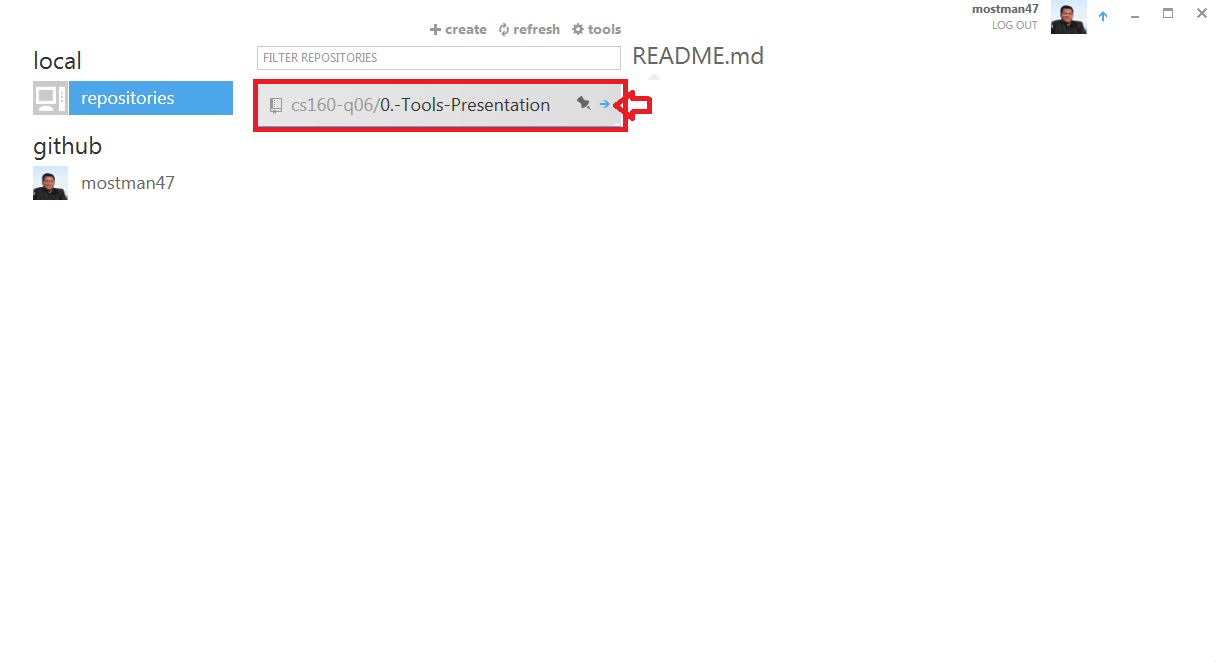
\includegraphics[width=0.7\textwidth]{Screenshots/github/github4.png}
  \caption{Manage and Commit Repo}
\end{figure}
}
\frame{
  \transdissolve[duration=0.25]
  \frametitle{Software hosting facilities}
    {\Huge GitHub client installation} \\[1em]
   \begin{figure}[h!]   
      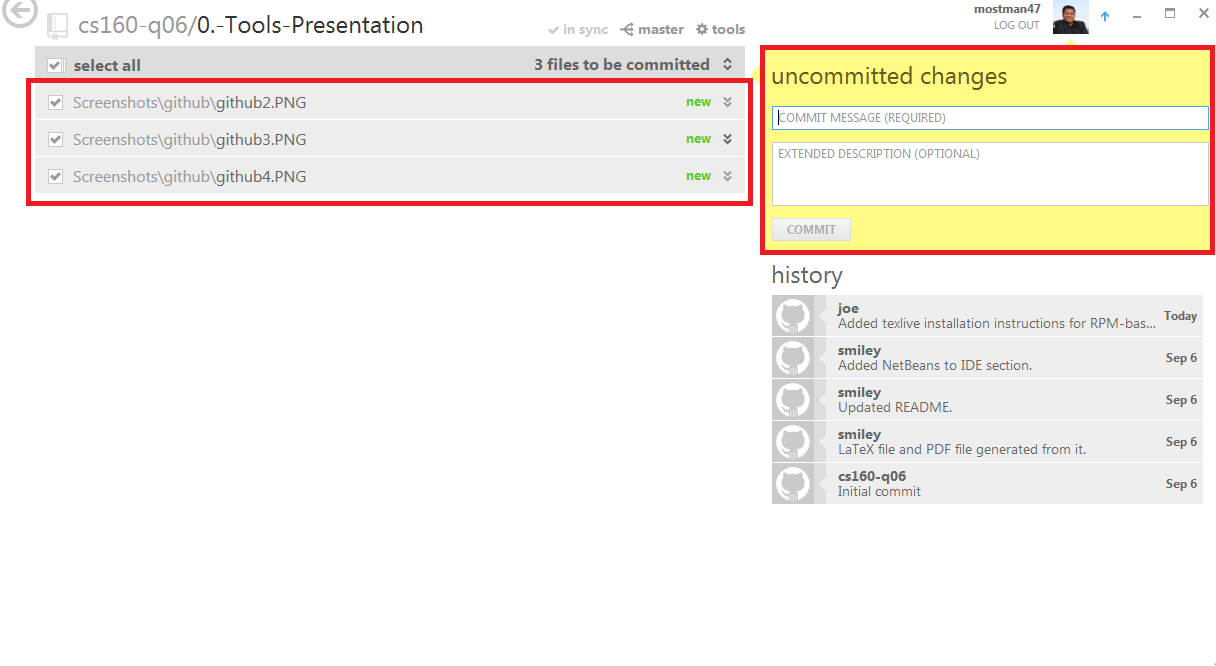
\includegraphics[width=0.7\textwidth]{Screenshots/github/github5.png}
  \caption{Manage and Commit Repo}
\end{figure}
}
\frame{
  \transdissolve[duration=0.25]
  \frametitle{Software hosting facilities}
    {\Huge GitHub client installation} \\[1em]
   \begin{figure}[h!]   
      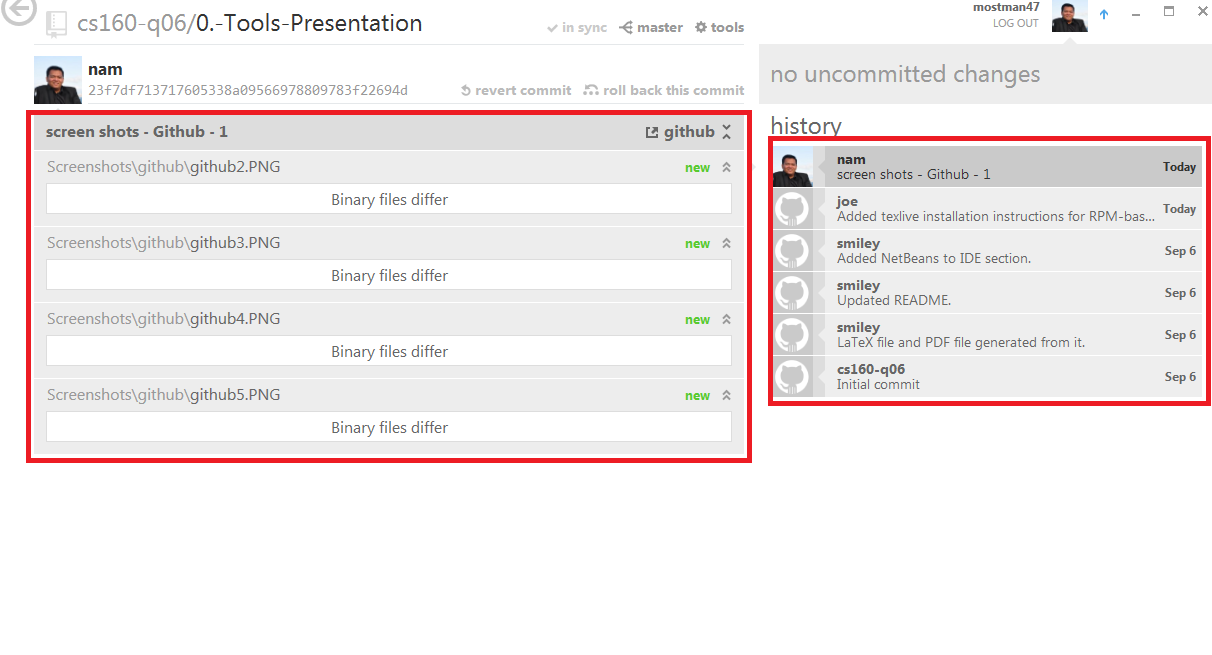
\includegraphics[width=0.7\textwidth]{Screenshots/github/github6.png}
  \caption{Result and History of Committing}
\end{figure}
}
%Codebeamer
\frame{
  \transdissolve[duration=0.25]
  \frametitle{Standalone bug trackers}
    {\Huge CodeBeamer} \\[1em] \pause 
    ``CodeBeamer is a web based Collaborative Application Lifecycle
    Management and Requirements management tool for distributed
    software development'' \\[2em] \pause
  \begin{itemize}
    \item Nonfree
    \item Backend: MariaDB (a.k.a. MySQL), Oracle, Apache Derby or
      PostgreSQL
    \item CodeBeamer is a collaborative Requirements Management (RM)
      and Application Lifecycle Management (ALM) solution for
      distributed software development.
  \end{itemize}
}

%Codebeamer compare
\frame{
  \transdissolve[duration=0.25]
  \frametitle{Standalone bug trackers}
    {\Huge CodeBeamer vs Others} \\[1em] \pause

  {\Large Bugzilla} \pause
  \begin{itemize}
  \item Licensed under the Mozilla Public License (a GNU
    GPL-compatible license, which means it is free software, so you
    have the freedom to run your own copy on your own server),
    developed/maintained by Mozilla Foundation.
  \item backend: MariaDB, Oracle, PostgreSQL, SQLite \pause
  \end{itemize}

  {\Large Google Code Hosting} \pause
  \begin{itemize}
  \item Not distributed as software that you can run on your own
    computer (hosted only); available for ``open source'' projects (by
    Google Code)
  \item BigTable backend (also proprietary)
  \end{itemize}
}

%Codebeamer installation
\frame{
  \transdissolve[duration=0.25]
  \frametitle{Standalone bug trackers}
    {\Huge CodeBeamer Installation} \\[1em] \pause
    \begin{figure}[h!]   
      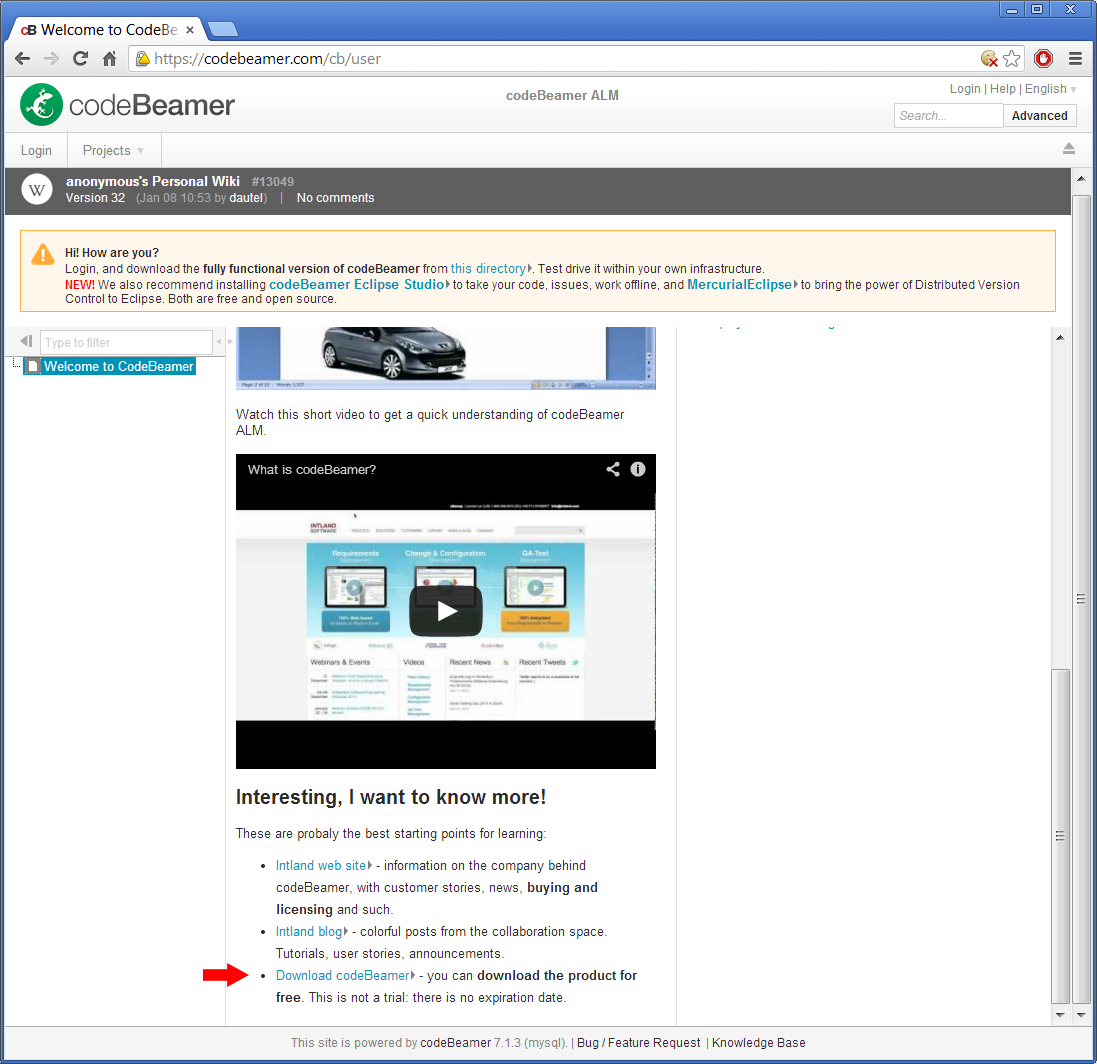
\includegraphics[width=0.7\textwidth]{Screenshots/codeBeamer/codeBeamer1.png}
      \caption{Download}
    \end{figure}
}

\frame{
  \transdissolve[duration=0.25]
  \frametitle{Standalone bug trackers}
    {\Huge CodeBeamer Installation} \\[1em]
    \begin{figure}[h!]
      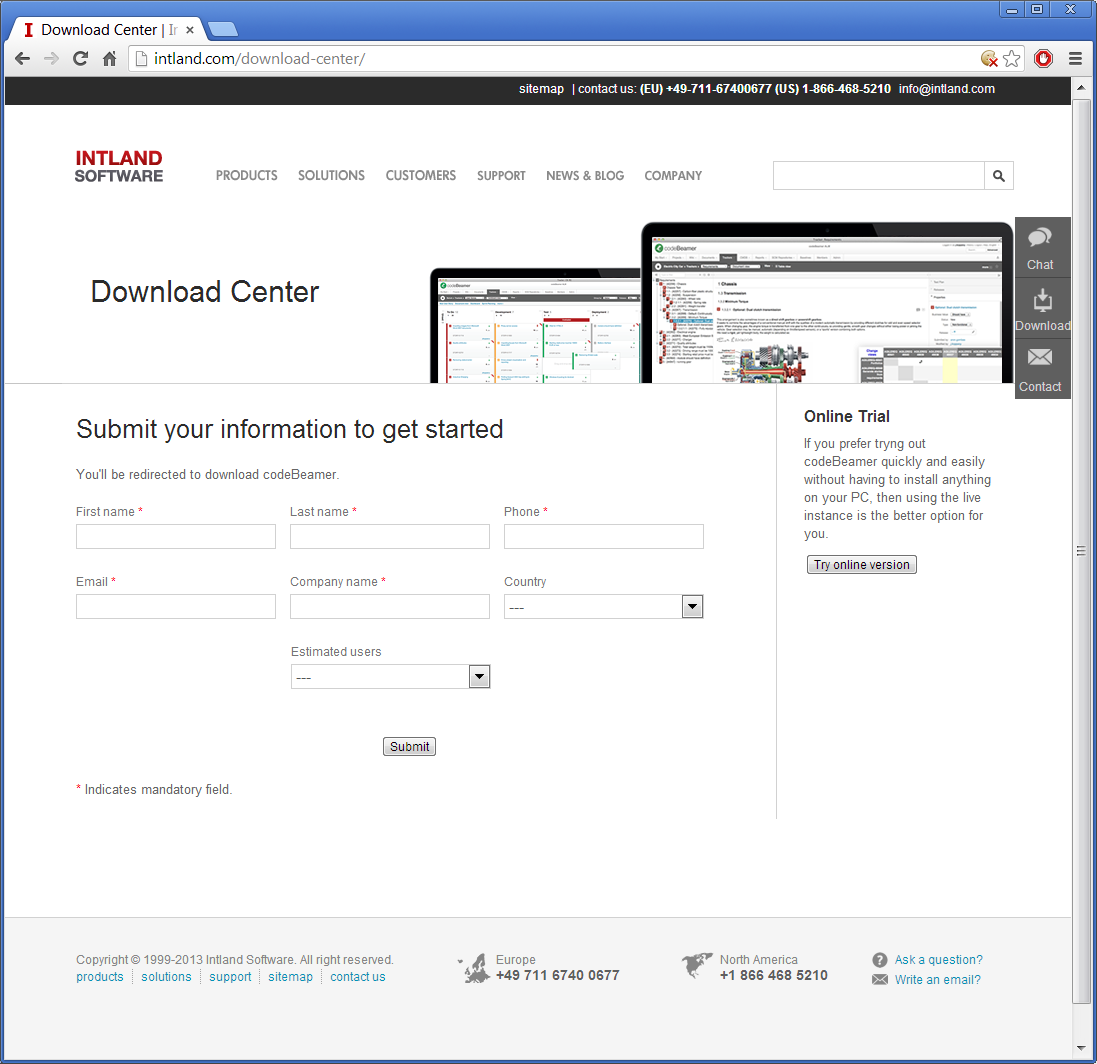
\includegraphics[width=0.7\textwidth]{Screenshots/codeBeamer/codeBeamer2.png}
      \caption{Download}
    \end{figure}   
}

\frame{
  \transdissolve[duration=0.25]
  \frametitle{Standalone bug trackers}
    {\Huge CodeBeamer Installation} \\[1em]
    \begin{figure}[h!]
      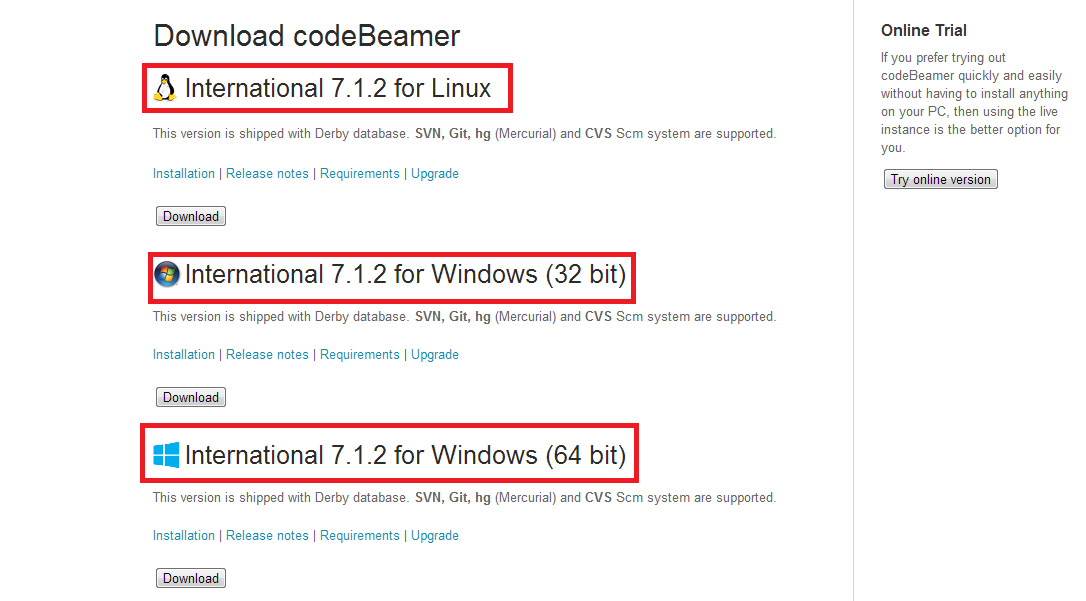
\includegraphics[width=0.7\textwidth]{Screenshots/codeBeamer/codeBeamer6.png}
      \caption{Download}
    \end{figure}   
}

\frame{
  \transdissolve[duration=0.25]
  \frametitle{Standalone bug trackers}
    {\Huge CodeBeamer Installation} \\[1em]
    \begin{figure}[h!]   
      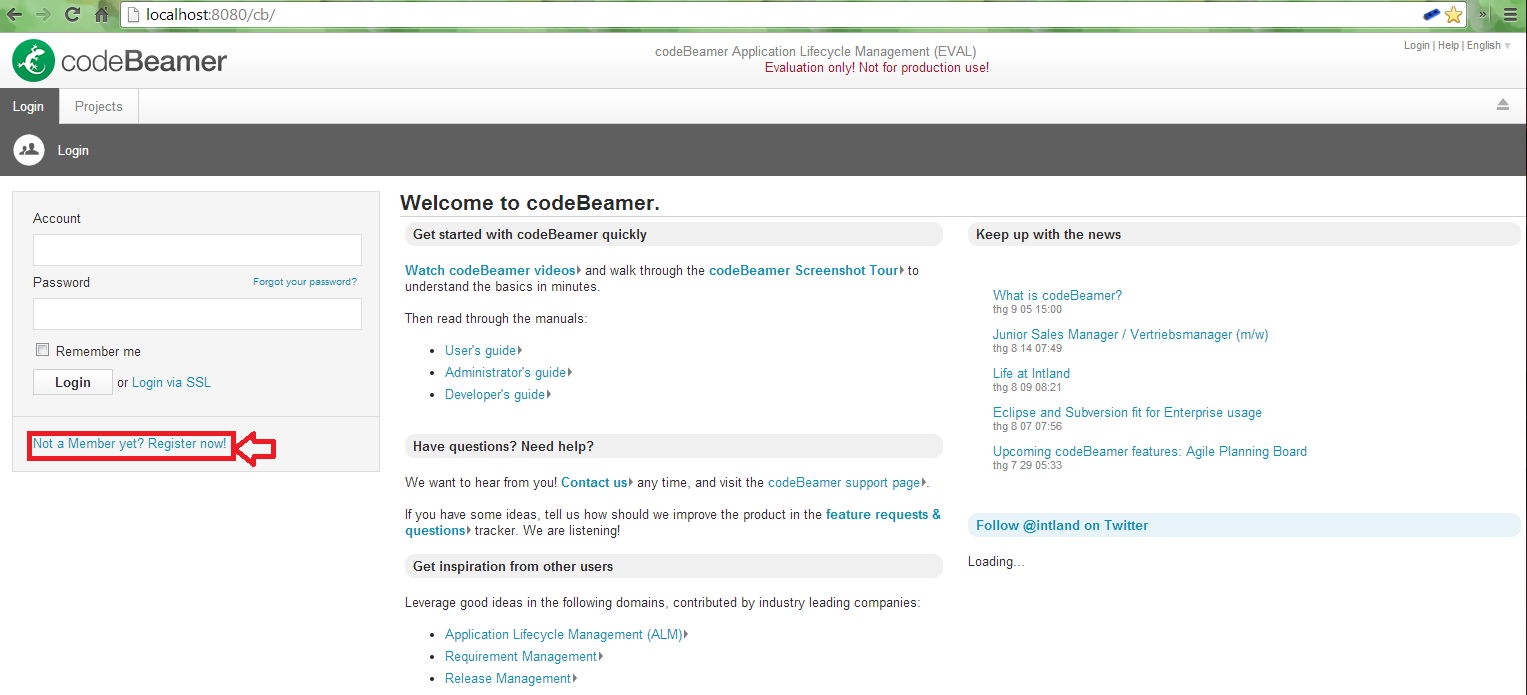
\includegraphics[width=0.7\textwidth]{Screenshots/codeBeamer/codeBeamer3.png}
      \caption{Web UI in localhost}
    \end{figure}
}

\frame{
  \transdissolve[duration=0.25]
  \frametitle{Standalone bug trackers}
    {\Huge CodeBeamer Installation} \\[1em]
    \begin{figure}[h!]   
      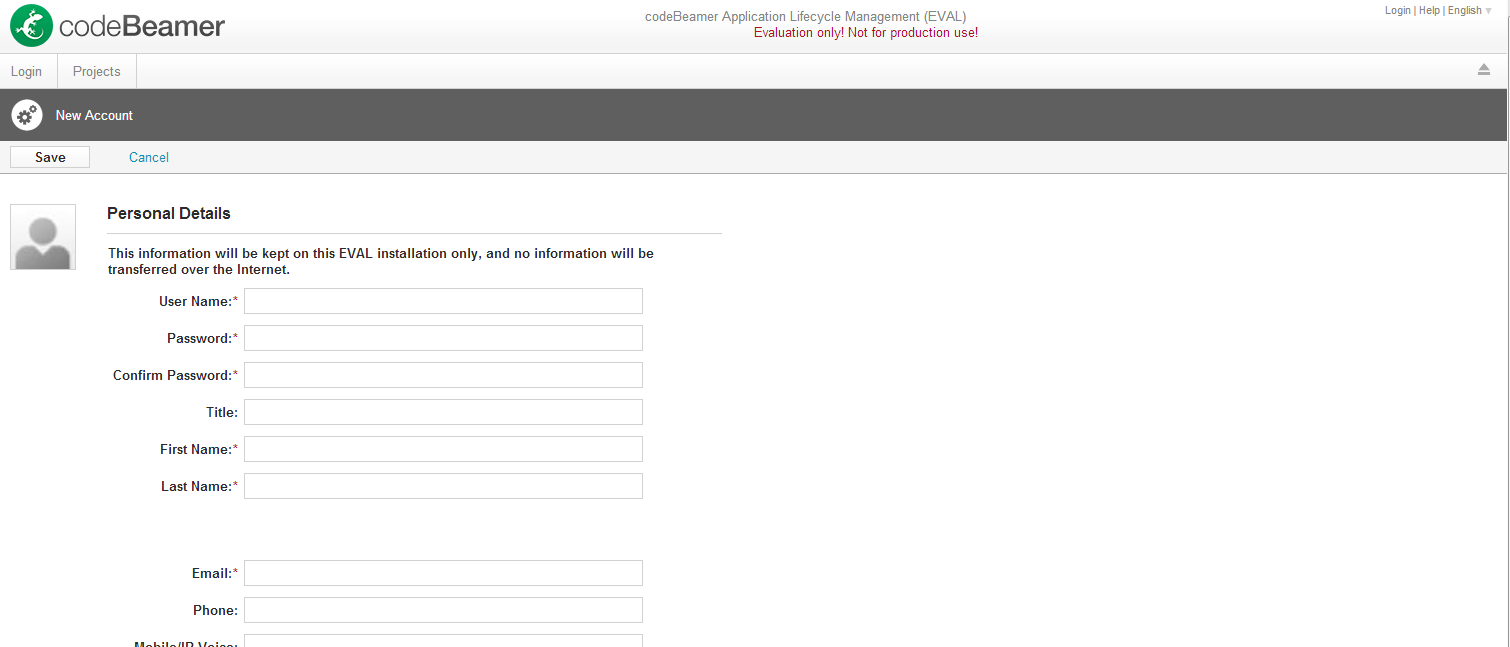
\includegraphics[width=0.7\textwidth]{Screenshots/codeBeamer/codeBeamer4.png}
      \caption{Register User}
    \end{figure}
}

\frame{
  \transdissolve[duration=0.25]
  \frametitle{Standalone bug trackers}
    {\Huge CodeBeamer Installation} \\[1em]
    \begin{figure}[h!]
      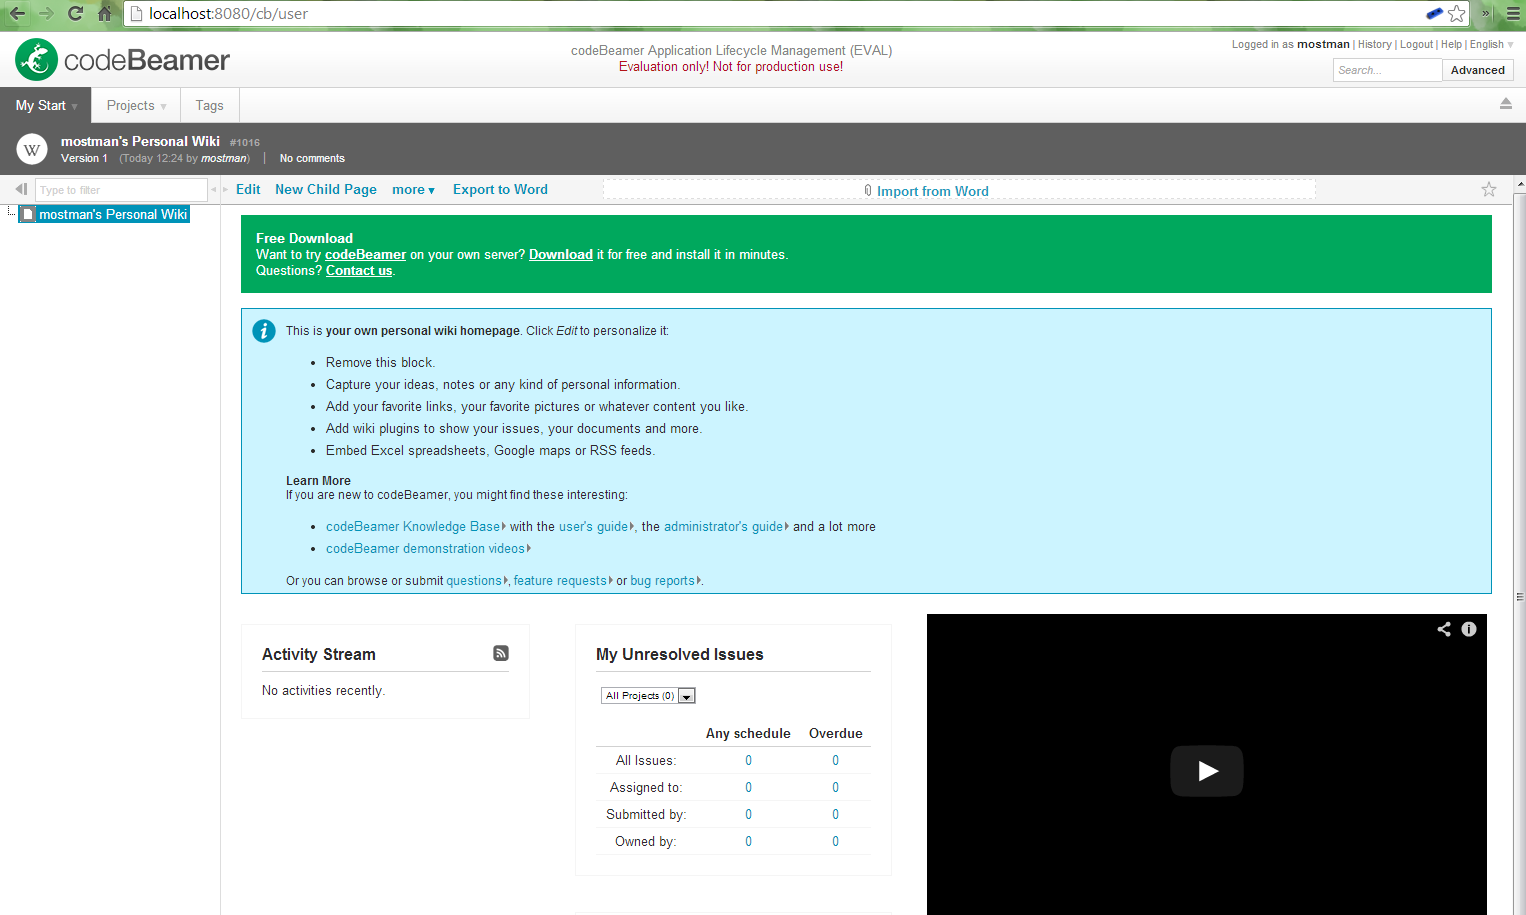
\includegraphics[width=0.7\textwidth]{Screenshots/codeBeamer/codeBeamer5.png}
      \caption{User's Management UI}
    \end{figure}
}

%IDEs: GNU Emacs
\frame{
  \transdissolve[duration=0.25]
  \frametitle{Editors and IDEs}
  \framesubtitle{Netbeans, Eclipse, GNU Emacs}
  \begin{itemize}
    \item {\bf GNU Emacs}
      \pause
      \begin{itemize}
        \item License: GNU GPLv3
          \pause
        \item Text editor
          \pause
        \item Extensible
          \pause
        \item Customizable
      \end{itemize}
  \end{itemize}
}

%IDEs: Netbeans and Eclipse
\frame{
  \transdissolve[duration=0.25]
  \frametitle{Editors and IDEs}
  \framesubtitle{Netbeans, Eclipse, Emacs} \pause
    \begin{itemize}
    \item {\bf NetBeans IDE} \pause
      \begin{itemize}
        \item Dual-licensed under Common Development and Distribution
          License (CDDL) v1.0 and GNU GPLv2, with some components
          released other third-party licenses \pause
        \item Create and debug rich web and mobile applications using
          the latest HTML5, \pause JavaScript, \pause and CSS3
          standards.  \pause
        \item Page inspector \pause
        \item CSS style editor \pause
        \item JavaScript editor \pause
        \item JavaScript debugger \pause
        \item Support for PHP, Java, C, C++ \pause
      \end{itemize}
    \item {\bf Eclipse} \pause
      \begin{itemize}
        \item License: MPL \pause
        \item IDE framework \pause
        \item Tools framework \pause \\[1em]
      \end{itemize}
    \end{itemize}
}

%Eclipse Installation
\frame{
  \transdissolve[duration=0.25]
  \frametitle{Editors and IDEs}
  \framesubtitle{http://www.eclipse.org/downloads/}
    {\Huge Eclipse Installation} \pause \\[1em]
    \begin{figure}[h!]   
      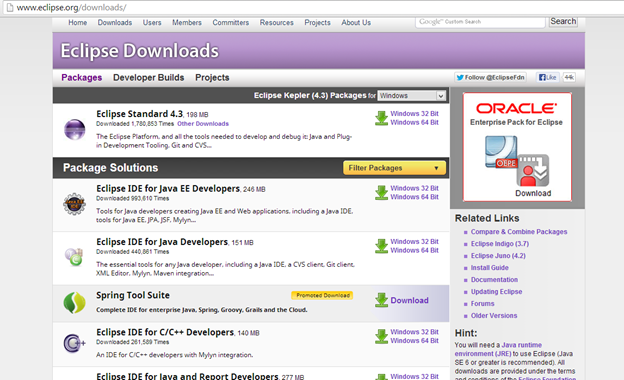
\includegraphics[width=0.7\textwidth]{Screenshots/eclipse/eclipse1.png}
      \caption{Download}
    \end{figure}
}

\frame{ \transdissolve[duration=0.25] 
  \frametitle{Editors and IDEs}
    {\Huge Eclipse Installation}\\[1em]
    \begin{figure}[h!]   
      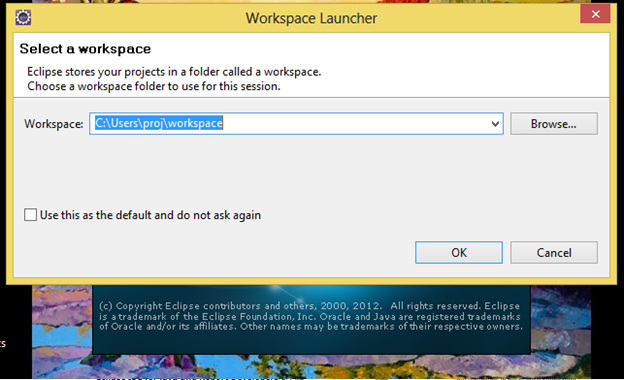
\includegraphics[width=0.7\textwidth]{Screenshots/eclipse/eclipse2.png}
      \caption{Workspace}
    \end{figure}
}

\frame{ \transdissolve[duration=0.25] 
  \frametitle{Editors and IDEs}
    {\Huge Eclipse Installation}\\[1em]
    \begin{figure}[h!]   
       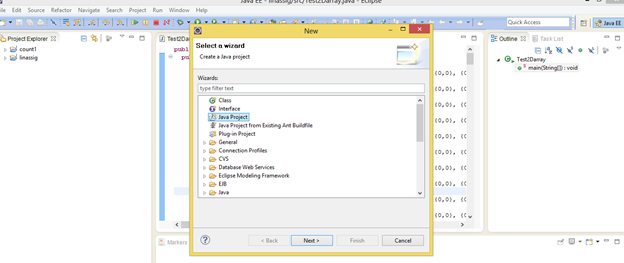
\includegraphics[width=0.7\textwidth]{Screenshots/eclipse/eclipse3.png}
      \caption{Create new project}
     \end{figure}
}

\frame{
  \transdissolve[duration=0.25]
  \frametitle{Editors and IDEs}
    {\Huge Eclipse Installation}\\[1em]
    \begin{figure}[h!]   
       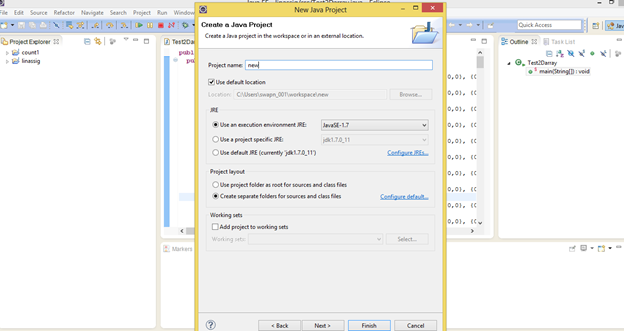
\includegraphics[width=0.7\textwidth]{Screenshots/eclipse/eclipse4.png}
      \caption{Create new project}
     \end{figure}
}

\frame{ \transdissolve[duration=0.25]
  \frametitle{Editors and IDEs}
    {\Huge Eclipse Installation}\\[1em]
    \begin{figure}[h!]   
      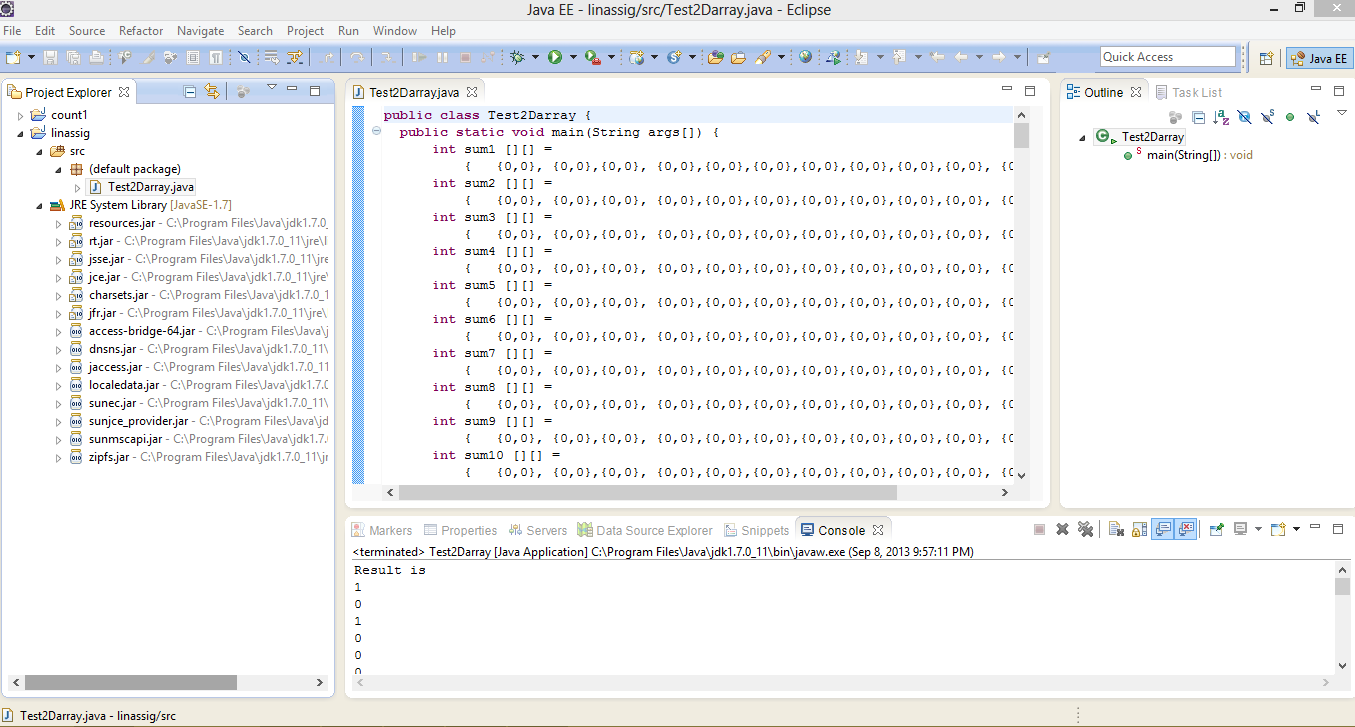
\includegraphics[width=0.7\textwidth]{Screenshots/eclipse/eclipse6.png}
      \caption{Running Program}
    \end{figure}
}

\frame{ \transdissolve[duration=0.25]
  \frametitle{Editors and IDEs}
    {\Huge Eclipse Installation}\\[1em]
    \begin{figure}[h!]   
      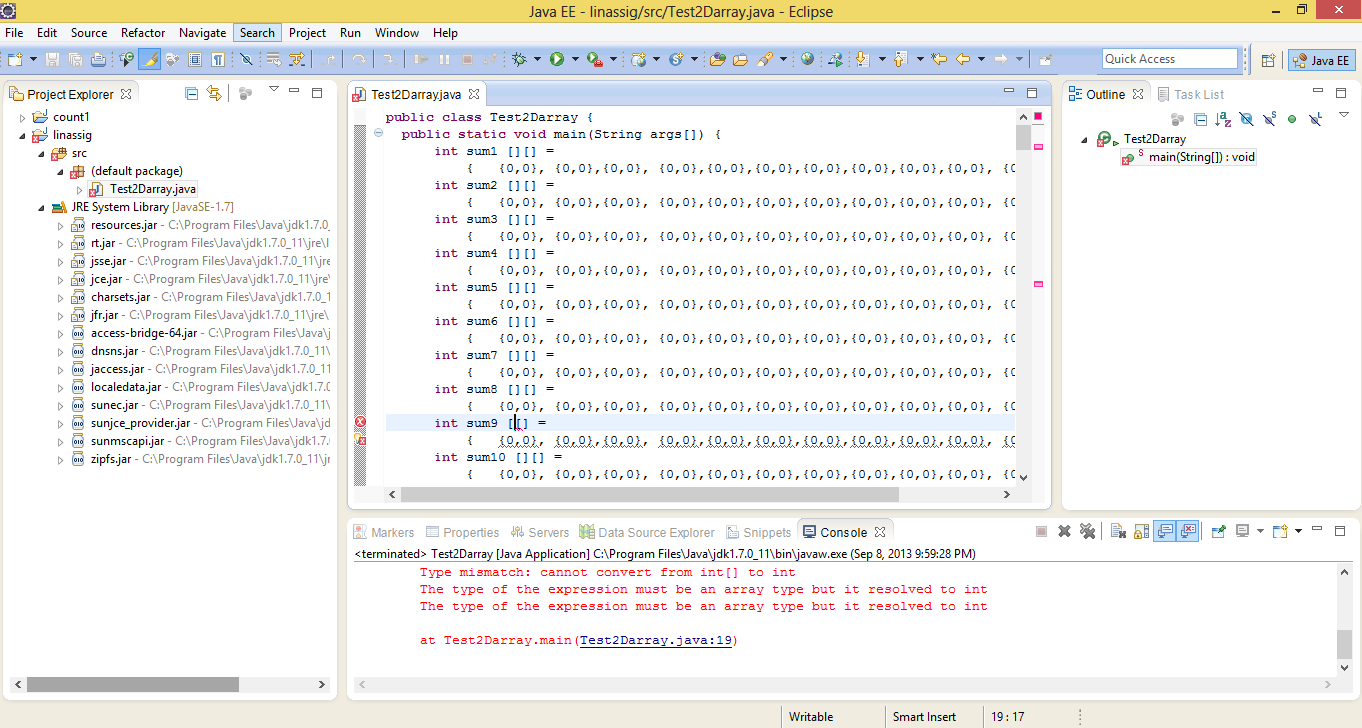
\includegraphics[width=0.7\textwidth]{Screenshots/eclipse/eclipse5.png}
      \caption{Error Logs}
    \end{figure}
}
%OpenProj
\frame{ \transdissolve[duration=0.25]
  \frametitle{Project Management Tools}
    {\Huge OpenProj}\\[1em] \pause 
    ``OpenProj is an open source project management software
    application. It intends to be a complete desktop replacement for
    Microsoft Project. It runs on the Java platform, allowing it to
    run on a variety of different operating systems''\\[2em] \pause
    \begin{itemize}
    \item License: Free, open source project management application
      that supports project timelines, issue tracking, wiki, document
      management, time and cost reporting, code management, Scrum, and
      more.
    \item Earned Value costing
    \item Gantt chart      
    \item Resource Breakdown Structure (RBS) chart
    \end{itemize}
}

%OpenProj vs. Microsoft Project
\frame{ \transdissolve[duration=0.25]
  \frametitle{Project Management Tools}
    {\Huge OpenProj vs. Microsoft Project}\\[1em]
    \pause
  {\Large Similar}
  \begin{itemize}
  \item user interface and approach to construction of project plan
  \item create workbench breakdown structure
  \item assign resources \pause
      \end{itemize}
          {\Large Different}
          \begin{itemize}
    	  \item OpenProj can link upwards with methods (inserting tasks is more difficult than with Microsoft Project)
            
          \item OpenProj can just create resources (have to do so in the resource sheet)
          \item OpenProj lacks a more detailed view and project reports that is available with Microsoft Project  
            
          \end{itemize}
}
%OpenProj installation
\frame{
  \transdissolve[duration=0.25]
  \frametitle{Project Management Tools}
    {\Huge OpenProj Installation}\\[1em]
    \pause
     \begin{figure}[h!]   
      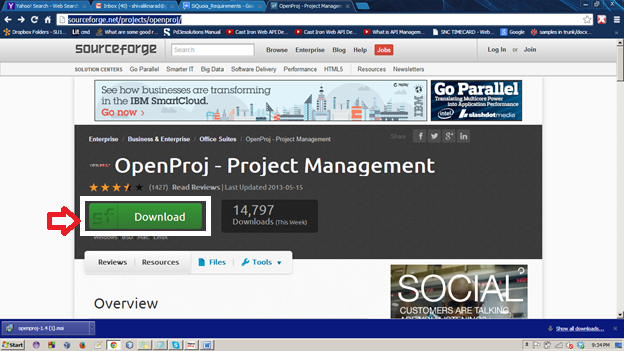
\includegraphics[width=0.7\textwidth]{Screenshots/openProj/openProj1.png}
  \caption{Download}
\end{figure}
   
}
\frame{ \transdissolve[duration=0.25]
  \frametitle{Project Management Tools}
    {\Huge OpenProj Installation}\\[1em]
    \begin{itemize}
    \item Step 1 – Double click and open the downloaded file. A dialog
      box will appear.
    \item Step 2 – Hit run button on the dialog box.
    \item Step 3 – Choose the directory where you want to install. And
      click next.
    \item Step 4 – click install
    \item Step 5 – click Finish. And your installation will be
      complete.
    \end{itemize}
} 

\frame{ \transdissolve[duration=0.25] 
  \frametitle{Project Management Tools}
    {\Huge OpenProj Installation}\\[1em]
    \begin{figure}[h!]   
      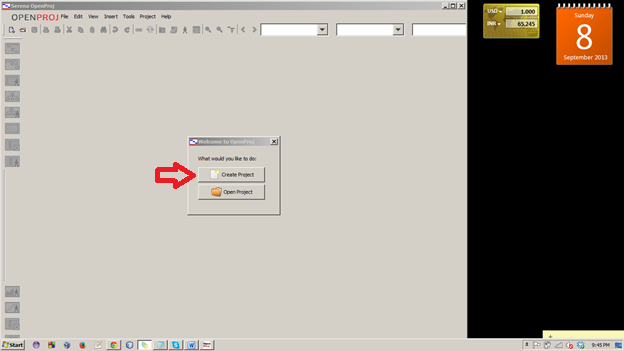
\includegraphics[width=0.7\textwidth]{Screenshots/openProj/openProj2.png}
      \caption{OpenProj's UI}
    \end{figure}
}

\frame{ \transdissolve[duration=0.25]
  \frametitle{Project Management Tools}
    {\Huge OpenProj Installation}\\[1em]
    \begin{figure}[h!]   
      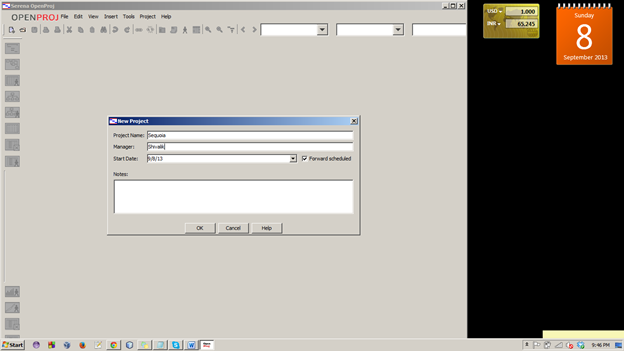
\includegraphics[width=0.7\textwidth]{Screenshots/openProj/openProj3.png}
      \caption{Create new Project}
    \end{figure}
}

\frame{ \transdissolve[duration=0.25]
  \frametitle{Project Management Tools}
    {\Huge OpenProj Installation}\\[1em]
    \begin{figure}[h!]   
      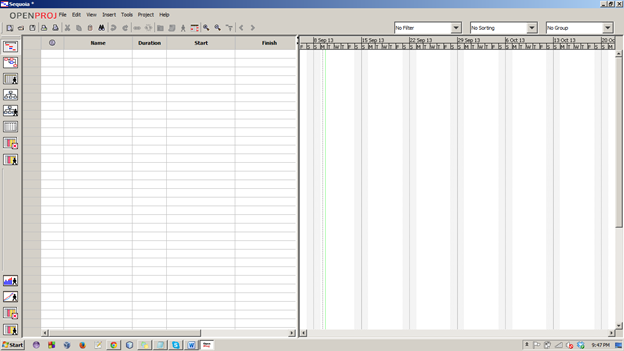
\includegraphics[width=0.7\textwidth]{Screenshots/openProj/openProj4.png}
      \caption{A project with empty sheet}
    \end{figure}
}

\frame{ \transdissolve[duration=0.25]
  \frametitle{Project Management Tools}
    {\Huge OpenProj Installation}\\[1em]
    \begin{figure}[h!]   
      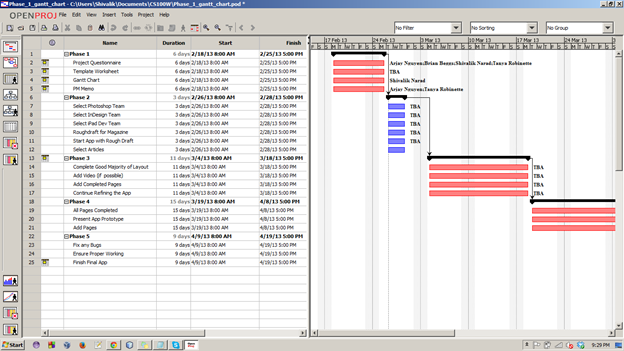
\includegraphics[width=0.7\textwidth]{Screenshots/openProj/openProj5.png}
      \caption{A project with details and timeline}
    \end{figure}
}

%References
\begin{frame}
  \transdissolve[duration=0.25]
  \frametitle{References}

  \begin{thebibliography}{10}
  \bibitem{RCS} {\tiny
          http://en.wikipedia.org/wiki/Comparison\_of\_revision\_control\_software}
  \bibitem{hosting} {\tiny
          http://en.wikipedia.org/wiki/Comparison\_of\_open-source\_software\_hosting\_facilities}
  \bibitem{bugtracking} {\tiny
          http://en.wikipedia.org/wiki/Comparison\_of\_issue-tracking\_systems}
  \bibitem{proj} {\tiny
          http://en.wikipedia.org/wiki/OpenProj\#Comparison\_to\_Microsoft\_Project}
  \bibitem{git} {\tiny http://looble.org/git-vs-svn-which-is-better/}
  \bibitem{eclipse} {\tiny
          http://slashdot.org/topic/bi/visual-studio-vs-eclipse-a-programmers-matchup/}
  \bibitem{java} {\tiny
          http://www.programmers.kz/programming/java/articles\_java/14715-some-background-information-on-java-and-object-orientation.html}
  \end{thebibliography}
\end{frame}

\frame{ \transdissolve[duration=0.25]
  {\centering
    \begin{tabular}{l}
      {\Huge Team Q 06} \\[.5em]
      {\Huge thanks you\ldots}
    \end{tabular}
  }
}

\end{document}
